\documentclass{article}

\usepackage{amsmath}
\usepackage{amsfonts}
\usepackage{amssymb}
\usepackage{amsthm}
\usepackage{graphicx}
\usepackage{subcaption}
\usepackage{siunitx}
\usepackage[margin=0.5in]{geometry}
\usepackage{csvsimple}

\title{Homework 5}
\author{Miguel Angel Gomez Barrera}

\begin{document}
	\maketitle
\paragraph{1.} Simulate $10000$ coin tosses using your own LCG between $u \sim [0,1]$. Heads occur when $u \leq 0.5$ and Tails when $u > 0.5$. Create the following histograms:
\begin{itemize}
	\item \textit{(5 Points)} The results of all the tosses.
	\item \textit{(5 Points)} Pairs, i.e., $(x_n, x_{n+1}), (x_{n+2}, x_{n+3})$, etc.
	\item \textit{(5 Points)} Triplets, i.e.,$(x_n, x_{n+1}), (x_{n+2})$.
	\item \textit{(5 Points)} For the streaks, i.e., a run of $k$ for 'heads' is $k$ occurrences of heads in succession (and the next trial is 'tails').
	\item \textit{(5 Points)} Can you see any pattern? Comment on your result.
\end{itemize}
\paragraph{Solution} After simulating $10000$ tosses with a LCG with the following parameters:
$$x_0 = 5003, a = 9973, c = 9929, m = 9277.$$
\paragraph{}On the first experiment, we obtained for heads $5098$, and for tails $4902$, immediately we can observe an impact on the coin tossing distribution (CTD)
\begin{center}
	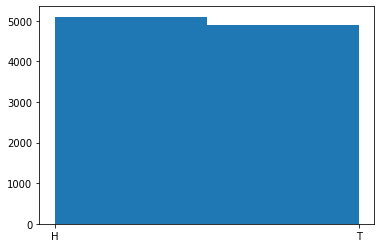
\includegraphics[width=0.4\linewidth]{all.png}
\end{center}
\paragraph{} as we can see it is very little, from now on we denote Heads with 'H' and Tails 'T'. We can compute the probability of each event separately and obtain that the chance of getting heads is $0.5098$ and tails $0.4902$, our random experiment was expected to have a similar behavior on fair coin (both results heads or tails have the same probability), but instead turns towards heads.
\paragraph{} The second experiment proposes to simulate two coins using the previous results, we obtain:
\begin{center}
	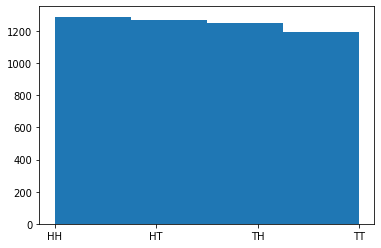
\includegraphics[width=0.4\linewidth]{pairs.png}
\end{center}
\paragraph{}As we see on the previous result, a combination that has heads has a greater probability to occur, also notice that we graph 'HT' and 'TH' as different results, if we treat these events as independent the analytical result will give us $0.25$, the probability values are:
\begin{center}
	\csvautotabular{pairs}
\end{center}
\paragraph{}On the previous experiment we did not analyze the difference, but we can say that it is similar: $+0.0098$ and $-0.0098$ for heads and tails respectively, but this time on some events the error was even less than in the previous, but it is greater on the combination that only has tails, we can infer that there is a bias on the algorithm.
\paragraph{} The next experiment is with three coins using the initial results.
\begin{center}
	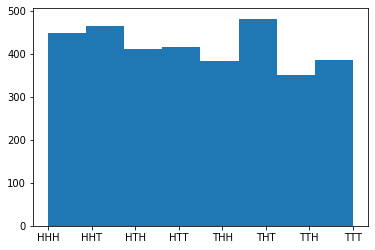
\includegraphics[width=0.4\linewidth]{triplets.png}
\end{center}
\begin{center}
	\csvautotabular{triplets}
\end{center}
\paragraph{} Our hypothesis of a bias seems to be true, even on other experiments, notice that the pair 'HHT' has a greater error than 'HTT', but by what we saw on the first experiment as we have an increment in Heads and a decrease in Tails, will imply that some combinations such as 'HHT' will have an excess of 'H's and a lack of 'T's to form the desired combination, the analytical difference tells us that, when is negative we lack the number of expected combination, and a positive value means that we have an excess of an expected combination. But what happens if the experiment is only dependend of our bias value? The next experiment will tell us.
\begin{center}
	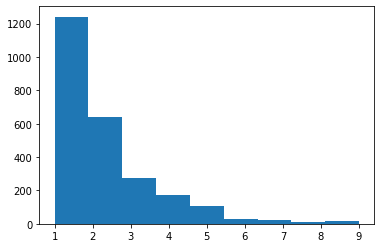
\includegraphics[width=0.4\linewidth]{streak.png}
\end{center}
\paragraph{}As expected, as the number of streak increases, it is more difficult to get an streak, but the data shows an ackward situation, actually it is easier to get a streak of 9 than a streak of 8, I'am currently not sure how to compute the analytical probability but this probably is related to the fact that the distribution has more heads than tails.
\begin{center}
	\csvautotabular{streak}
\end{center}
\paragraph{}The code to generate this graphsis called \textit{RunMeInPython.py}.
\paragraph{2.} Crack the following sequence:
$$[137, 553, 990, 881, 646, 618, 323, 832, 897, 230, 181, 432, 44, 925, 525, 695, 367, 711, 974, 274]$$
\paragraph{Solution.} For the LCG
$$X_n =  X_{n-1}a + c \pmod{m},$$
the parameters are:
$$a=997, c= 23, m= 1023,$$
\paragraph{}The codefile is named \textit{2.py}.
\end{document} 